%%%%%%%%%%%%%%%%%%%%%%%%%%%%%%%%%%%%%%%%%%%%%%%%%%%%%%%%%%%%%%%%%%%%%%%%%%%%%%%%%%
\begin{frame}[fragile]\frametitle{}
\begin{center}
{\Large Introduction}
\end{center}
\end{frame}

%%%%%%%%%%%%%%%%%%%%%%%%%%%%%%%%%%%%%%%%%%%%%%%%%%%%%%%%%%%%%%%%%%%%%%%%%%%%%%%%%%
\begin{frame}[fragile]\frametitle{}
\begin{center}
{\Large Practical Scenario}
\end{center}
\end{frame}

%%%%%%%%%%%%%%%%%%%%%%%%%%%%%%%%%%%%%%%%%%%%%%%%%%%%%%%%%%%%%%%%%%%%%%%%%%%%%%%%%
\begin{frame}[fragile]\frametitle{Icertis Discover AI}
\begin{columns}
    \begin{column}[T]{0.6\linewidth}
      \begin{center}
      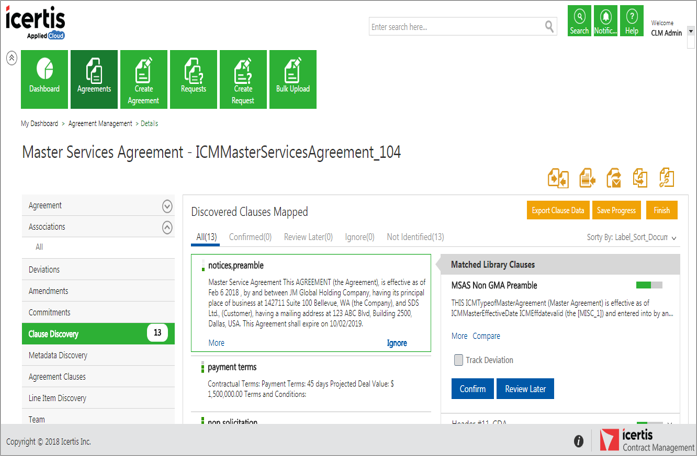
\includegraphics[width=\linewidth,keepaspectratio]{xai1}
	  	\end{center}
    \end{column}
    \begin{column}[T]{0.4\linewidth}

			
				\begin{itemize}
				\item Image/PDF Conversion
				\item Clause Discovery, by Delineation and Classification
				\item Attribute Discovery, by NER
				\item Tables Discovery, Image processing
				\end{itemize}
    \end{column}
  \end{columns}
  
\tiny{(Ref: https://www.icertis.com/contract-management-software/ai-applications/discoverai/ )}
\end{frame}

%%%%%%%%%%%%%%%%%%%%%%%%%%%%%%%%%%%%%%%%%%%%%%%%%%%%%%%%%%%
\begin{frame}[fragile]\frametitle{A Sample Digitization Project}
\begin{itemize}
\item Number of Contracts to be Digitized : 60K
\item Number of Clauses to be discovered : 32 (“Term”, “Warranty”, \ldots)
\item Number of Attributes to be discovered: 12 (“Effective Date”, “Contract Value”,\ldots)
\item Time : 3 months

\end{itemize}
\end{frame}

%%%%%%%%%%%%%%%%%%%%%%%%%%%%%%%%%%%%%%%%%%%%%%%%%%%%%%%%%%%
\begin{frame}[fragile]\frametitle{Steps}
\begin{itemize}
\item Build AI Engine using annotated samples to extract attributes
\item Show results of training to the Customer and get approval
\item Start extractions (production) for all the contracts, in batches \ldots
\end{itemize}
\end{frame}

%%%%%%%%%%%%%%%%%%%%%%%%%%%%%%%%%%%%%%%%%%%%%%%%%%%%%%%%%%%%%%%%%%%%%%%%%%%%%%%%%%
\begin{frame}[fragile]\frametitle{}
\begin{center}
{\Large Halfway through the production \ldots}
\end{center}
\end{frame}

%%%%%%%%%%%%%%%%%%%%%%%%%%%%%%%%%%%%%%%%%%%%%%%%%%%%%%%%%%%
\begin{frame}[fragile]\frametitle{A sample dialog}
\begin{itemize}
\item {\bf Customer}: The extractions are looking ok, but \ldots
\item {\bf AIML team}: But??
\item {\bf Customer}: Why are you digitizing these ‘DELLA' contracts?
\item {\bf AIML team}: Meaning?
\item {\bf Customer}: You should not digitize contracts having ‘DELLA Corporation' in the footer.
\item {\bf AIML team}: But you never told us. No mention of any such rules in SOW also..
\item {\bf Customer}: We are just asking you to NOT process these, not adding to your work/scope!!
\item {\bf AIML team}: But \ldots
\item {\bf Customer}: Shouldn't be difficult, right? AI will find out \ldots

\end{itemize}
\end{frame}

%%%%%%%%%%%%%%%%%%%%%%%%%%%%%%%%%%%%%%%%%%%%%%%%%%%%%%%%%%%%%%%%%%%%%%%%%%%%%%%%%%
\begin{frame}[fragile]\frametitle{}
\begin{center}
(we keep hearing \ldots)


{\Huge AI {\bf will} find out!!}
\end{center}
\end{frame}


%%%%%%%%%%%%%%%%%%%%%%%%%%%%%%%%%%%%%%%%%%%%%%%%%%%%%%%%%%%%%%%%%%%%%%%%%%%%%%%%%%
\begin{frame}[fragile]\frametitle{}
\begin{center}
(sometimes \ldots)


{\Huge AI {\bf should} find out!!}
\end{center}
\end{frame}

%%%%%%%%%%%%%%%%%%%%%%%%%%%%%%%%%%%%%%%%%%%%%%%%%%%%%%%%%%%%%%%%%%%%%%%%%%%%%%%%%%
\begin{frame}[fragile]\frametitle{}
\begin{center}
(what if \ldots)


{\Huge AI {\bf can not} find out!!}
\end{center}
\end{frame}

%%%%%%%%%%%%%%%%%%%%%%%%%%%%%%%%%%%%%%%%%%%%%%%%%%%%%%%%%%%%%%%%%%%%%%%%%%%%%%%%%%
\begin{frame}[fragile]\frametitle{}
\begin{center}
(and worse, if \ldots)


{\Huge AI {\bf finds it and finds wrong stuff}!!}
\end{center}
\end{frame}

%%%%%%%%%%%%%%%%%%%%%%%%%%%%%%%%%%%%%%%%%%%%%%%%%%%%%%%%%%%%%%%%%%%%%%%%%%%%%%%%%%
\begin{frame}[fragile]\frametitle{}
\begin{center}
(bottom line… we need to understand that \ldots)


{\Huge AI {\bf is not Magic}!!}
\end{center}
\end{frame}

%%%%%%%%%%%%%%%%%%%%%%%%%%%%%%%%%%%%%%%%%%%%%%%%%%%%%%%%%%%%%%%%%%%%%%%%%%%%%%%%%%
\begin{frame}[fragile]\frametitle{}
\begin{center}
(But still, you need to explain me)


{\Huge Why AI gave this result!!}
\end{center}
\end{frame}

%%%%%%%%%%%%%%%%%%%%%%%%%%%%%%%%%%%%%%%%%%%%%%%%%%%%%%%%%%%%%%%%%%%%%%%%%%%%%%%%%%
\begin{frame}[fragile]\frametitle{}
\begin{center}
(that's)


{\Huge Explainable AI!!}
\end{center}
\end{frame}


%%%%%%%%%%%%%%%%%%%%%%%%%%%%%%%%%%%%%%%%%%%%%%%%%%%%%%%%%%
\begin{frame}[fragile]\frametitle{Need for Explainable AI}
\begin{center}
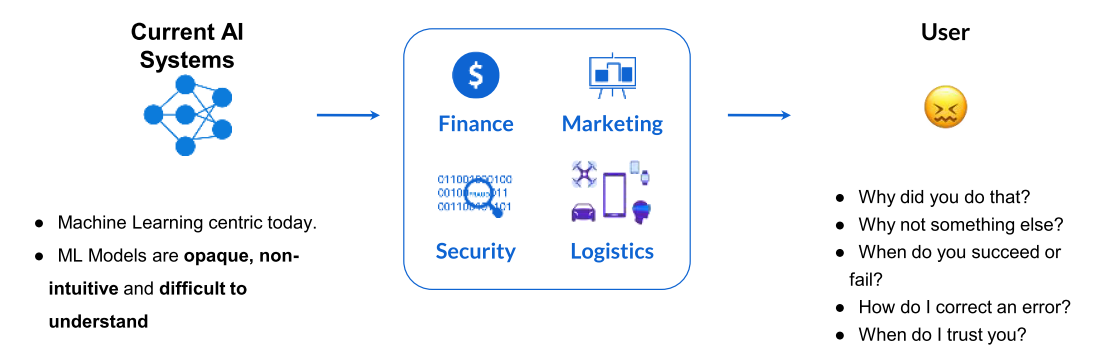
\includegraphics[width=\linewidth,keepaspectratio]{xai2}
\end{center}

Explainable AI is essential for customers to understand and trust the decisions by AI.

\tiny{(Ref: Explainable AI in Industry, KDD 2019 Tutorial,Sahin Cem Geyik, Krishnaram Kenthapadi \& Varun Mithal  )}

\end{frame}

%%%%%%%%%%%%%%%%%%%%%%%%%%%%%%%%%%%%%%%%%%%%%%%%%%%%%%%%%%
\begin{frame}[fragile]\frametitle{Wrong decisions: Costly and dangerous}
\begin{center}
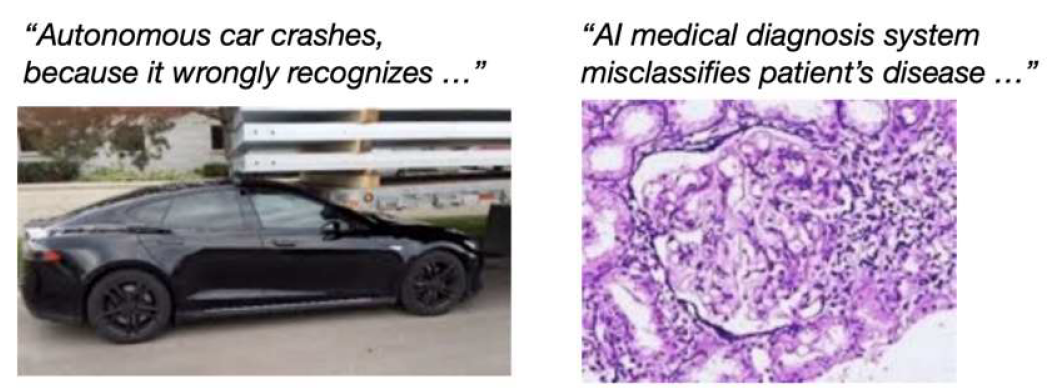
\includegraphics[width=\linewidth,keepaspectratio]{xai3}
\end{center}

\tiny{(Ref: Credit: Samek, Binder, Tutorial on Interpretable ML, MICCAI'18 )}

\end{frame}

%%%%%%%%%%%%%%%%%%%%%%%%%%%%%%%%%%%%%%%%%%%%%%%%%%%%%%%%%%%
\begin{frame}[fragile]\frametitle{AI as Black Box }
\begin{itemize}
\item Why did the AI system do that?
\item Why didn't the AI system do something else?
\item When did the AI system succeed?
\item When did the AI system fail?
\item When does the AI system give enough confidence in the decision that you can trust it?
\item How can the AI system correct an error?
\end{itemize}

\tiny{(Ref:Explainable AI (XAI) – A Perspective, Saurabh Kaushik  )}

\end{frame}

%%%%%%%%%%%%%%%%%%%%%%%%%%%%%%%%%%%%%%%%%%%%%%%%%%%%%%%%%%%%%%%%%%%%%%%%%%%%%%%%%%
\begin{frame}[fragile]\frametitle{}
\begin{center}
{\Large Need for Explainable AI}
\end{center}
\end{frame}

%%%%%%%%%%%%%%%%%%%%%%%%%%%%%%%%%%%%%%%%%%%%%%%%%%%%%%%%%%%
\begin{frame}[fragile]\frametitle{Gartner Hype Cycle 2019}

\begin{center}
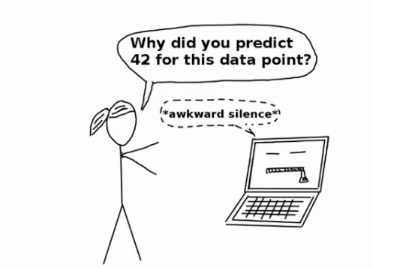
\includegraphics[width=0.8\linewidth,keepaspectratio]{xai24}

\tiny{(Ref: XAI - Udemy  )}
\end{center}
\end{frame}


%%%%%%%%%%%%%%%%%%%%%%%%%%%%%%%%%%%%%%%%%%%%%%%%%%%%%%%%%%%
\begin{frame}[fragile]\frametitle{Why Explainable AI?}
\begin{itemize}
\item As Machine Learning gets more prevalent, interpretation of results is needed by various stakeholders.
\item Regulatory compliance.
\item Insights into Black Box models.
\end{itemize}

\tiny{(Ref: XAI - Udemy  )}

\end{frame}

%%%%%%%%%%%%%%%%%%%%%%%%%%%%%%%%%%%%%%%%%%%%%%%%%%%%%%%%%%%
\begin{frame}[fragile]\frametitle{Three Key Pillars of Explainable AI}
\begin{itemize}
\item {\bf Reasonable AI}: The ability to understand the reasoning behind each individual prediction
\item {\bf Traceable AI}: The ability to trace prediction process from algorithm to data. 
\item {\bf Understandable AI}: The ability to fully understand the AI decision-making is based

\end{itemize}

\tiny{(Ref:Explainable AI (XAI) – A Perspective, Saurabh Kaushik  )}

\end{frame}

%%%%%%%%%%%%%%%%%%%%%%%%%%%%%%%%%%%%%%%%%%%%%%%%%%%%%%%%%%%
\begin{frame}[fragile]\frametitle{Business Benefits}
“Explainable AI is Responsible AI”

\begin{center}
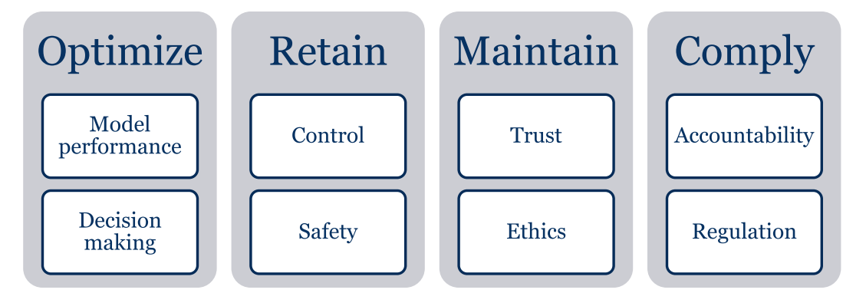
\includegraphics[width=\linewidth,keepaspectratio]{xai4}
\end{center}

“Right to Explanation” – GDPR 

\tiny{(Ref:Explainable AI (XAI) – A Perspective, Saurabh Kaushik  )}

\end{frame}

%%%%%%%%%%%%%%%%%%%%%%%%%%%%%%%%%%%%%%%%%%%%%%%%%%%%%%%%%%%
\begin{frame}[fragile]\frametitle{Gartner Hype Cycle 2019}

\begin{center}
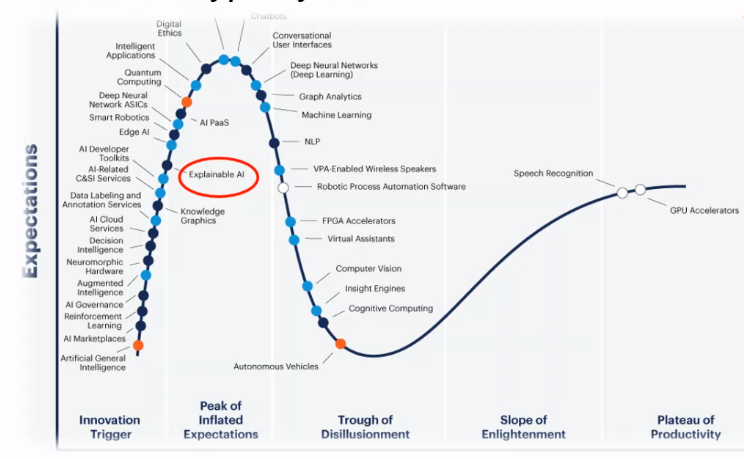
\includegraphics[width=0.8\linewidth,keepaspectratio]{xai23}
\end{center}


\tiny{(Ref: XAI - Udemy  )}

\end{frame}

%%%%%%%%%%%%%%%%%%%%%%%%%%%%%%%%%%%%%%%%%%%%%%%%%%%%%%%%%%%
\begin{frame}[fragile]\frametitle{Benefits of Explainable AI}
To increase:
\begin{itemize}
\item Trust and social acceptance
\item Transparency and detection of bias
\item Robustness and reliability of model (as we would be consistent in results even after slight perturbations in inputs)
\item Better understanding of the model and domain.
\end{itemize}

But it may reveal the commercial secrets !!

\tiny{(Ref: XAI - Udemy  )}

\end{frame}

%%%%%%%%%%%%%%%%%%%%%%%%%%%%%%%%%%%%%%%%%%%%%%%%%%%%%%%%%%%%%%%%%%%%%%%%%%%%%%%%%
\begin{frame}[fragile]\frametitle{Achieving Explainable AI}
\begin{columns}
    \begin{column}[T]{0.6\linewidth}
		Prediction explanations

				\begin{itemize}
				\item Important features
				\item Features weights
				\item Decision tree plotting
				\end{itemize}
				
    \end{column}
    \begin{column}[T]{0.4\linewidth}
		Build an interpretable model using libraries like LIME, SHAP, etc.

      \begin{center}
      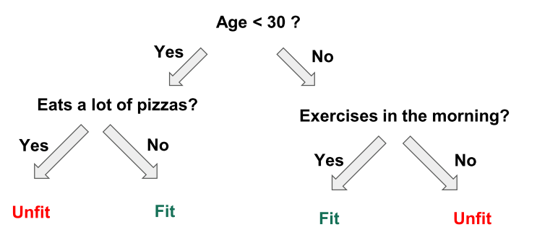
\includegraphics[width=\linewidth,keepaspectratio]{xai5}
	  	\end{center}
    \end{column}
  \end{columns}
  
\tiny{(Ref: Explainable AI in Industry, KDD 2019 Tutorial,Sahin Cem Geyik, Krishnaram Kenthapadi \& Varun Mithal)}
\end{frame}

%%%%%%%%%%%%%%%%%%%%%%%%%%%%%%%%%%%%%%%%%%%%%%%%%%%%%%%%%%%
\begin{frame}[fragile]\frametitle{}


\begin{center}
``Interpret-ability is the degree to which a human can 
understand the cause of a decision.''
\end{center}


\tiny{(Miller, Tim. 2017. ``Explanation in Artificial Intelligence: Insights from the Social Sciences'')}

\end{frame}

%%%%%%%%%%%%%%%%%%%%%%%%%%%%%%%%%%%%%%%%%%%%%%%%%%%%%%%%%%%%%%%%%%%%%%%%%%%%%%%%%%
\begin{frame}[fragile]\frametitle{}
\begin{center}
{\Large So, What (exactly) is AI?}
\end{center}
\end{frame}

%%%%%%%%%%%%%%%%%%%%%%%%%%%%%%%%%%%%%%%%%%%%%%%%%%%%%%%%%%%%%%%%%%%%%%%%%%%%%%%%%%
\begin{frame}[fragile]\frametitle{}
\begin{center}
(typical understanding)

{\Huge If Machines show intelligence, like Humans that's AI}
\end{center}
\end{frame}

%%%%%%%%%%%%%%%%%%%%%%%%%%%%%%%%%%%%%%%%%%%%%%%%%%%%%%%%%%
\begin{frame}[fragile]\frametitle{}
\begin{center}
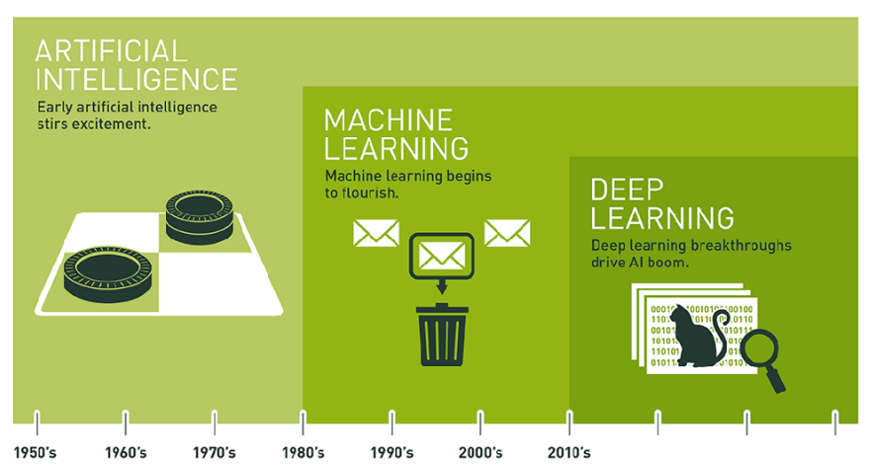
\includegraphics[width=\linewidth,keepaspectratio]{xai6}
\end{center}

\tiny{(Ref: Nvidia blog: Artificial Intelligence)}
\end{frame}

%%%%%%%%%%%%%%%%%%%%%%%%%%%%%%%%%%%%%%%%%%%%%%%%%%%%%%%%%%
\begin{frame}[fragile]\frametitle{Difference}
\begin{center}
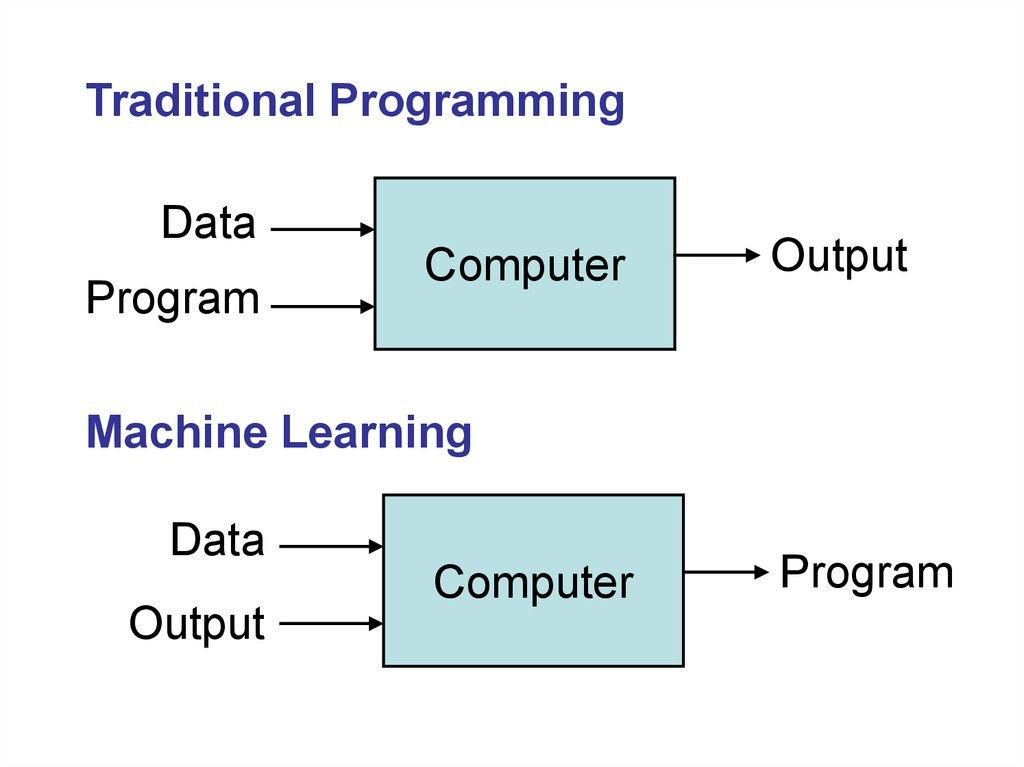
\includegraphics[width=0.8\linewidth,keepaspectratio]{xai7}
\end{center}

\tiny{(Ref: Machine Learning - Luis Serrano - Youtube)}
\end{frame}

%%%%%%%%%%%%%%%%%%%%%%%%%%%%%%%%%%%%%%%%%%%%%%%%%%%%%%%%%%
\begin{frame}[fragile]\frametitle{Supervised: Linear}
\begin{center}
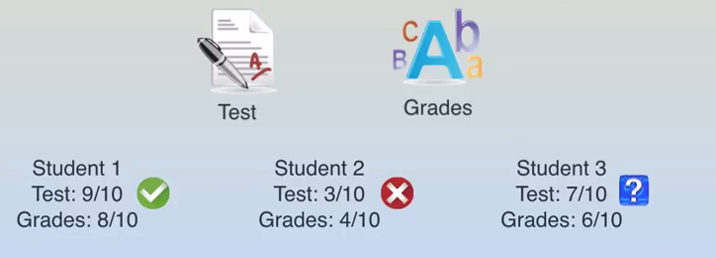
\includegraphics[width=\linewidth,keepaspectratio]{xai8}
\end{center}

\tiny{(Ref: Machine Learning - Luis Serrano - Youtube)}
\end{frame}

%%%%%%%%%%%%%%%%%%%%%%%%%%%%%%%%%%%%%%%%%%%%%%%%%%%%%%%%%%
\begin{frame}[fragile]\frametitle{Supervised: Linear}
\begin{center}
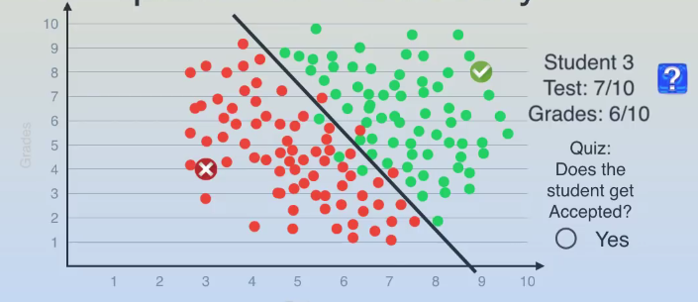
\includegraphics[width=\linewidth,keepaspectratio]{xai9}
\end{center}

\tiny{(Ref: Machine Learning - Luis Serrano - Youtube)}
\end{frame}

%%%%%%%%%%%%%%%%%%%%%%%%%%%%%%%%%%%%%%%%%%%%%%%%%%%%%%%%%%
\begin{frame}[fragile]\frametitle{Supervised: Non-Linear}
\begin{center}
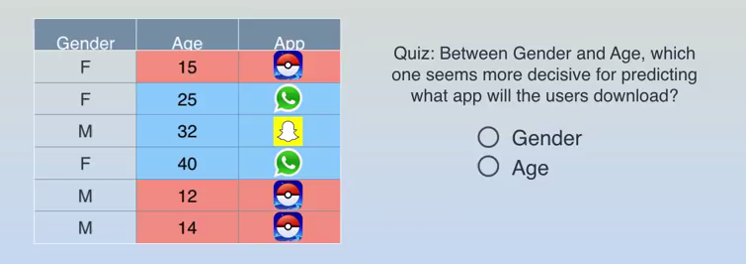
\includegraphics[width=\linewidth,keepaspectratio]{xai10}
\end{center}

\tiny{(Ref: Machine Learning - Luis Serrano - Youtube)}
\end{frame}

%%%%%%%%%%%%%%%%%%%%%%%%%%%%%%%%%%%%%%%%%%%%%%%%%%%%%%%%%%
\begin{frame}[fragile]\frametitle{Supervised: Non-Linear}
\begin{center}
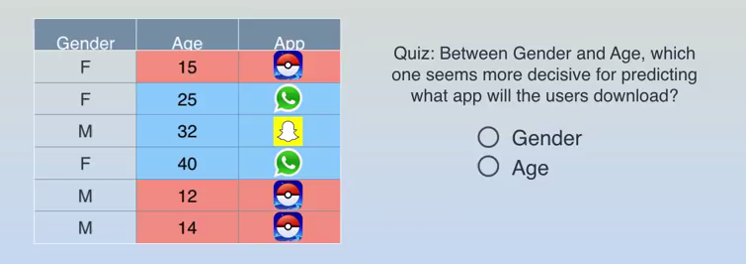
\includegraphics[width=\linewidth,keepaspectratio]{xai10}
\end{center}

\tiny{(Ref: Machine Learning - Luis Serrano - Youtube)}
\end{frame}

%%%%%%%%%%%%%%%%%%%%%%%%%%%%%%%%%%%%%%%%%%%%%%%%%%%%%%%%%%
\begin{frame}[fragile]\frametitle{Unsupervised}
\begin{center}
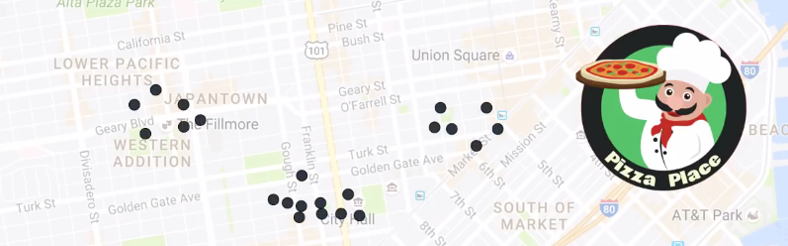
\includegraphics[width=\linewidth,keepaspectratio]{xai11}
\end{center}

\tiny{(Ref: Machine Learning - Luis Serrano - Youtube)}
\end{frame}

%%%%%%%%%%%%%%%%%%%%%%%%%%%%%%%%%%%%%%%%%%%%%%%%%%%%%%%%%%
\begin{frame}[fragile]\frametitle{Unsupervised}
\begin{center}
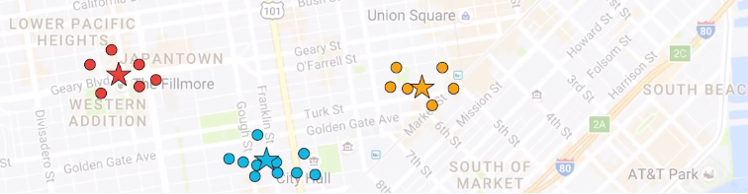
\includegraphics[width=\linewidth,keepaspectratio]{xai12}
\end{center}

\tiny{(Ref: Machine Learning - Luis Serrano - Youtube)}
\end{frame}

%%%%%%%%%%%%%%%%%%%%%%%%%%%%%%%%%%%%%%%%%%%%%%%%%%%%%%%%%%
\begin{frame}[fragile]\frametitle{How Neural Networks capture Non-Linearity?}
\begin{center}
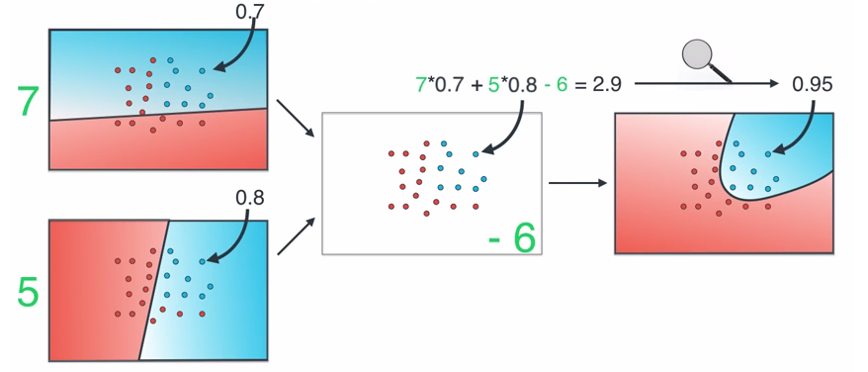
\includegraphics[width=\linewidth,keepaspectratio]{xai13}
\end{center}

\tiny{(Ref: Machine Learning - Luis Serrano - Youtube)}
\end{frame}

%%%%%%%%%%%%%%%%%%%%%%%%%%%%%%%%%%%%%%%%%%%%%%%%%%%%%%%%%%
\begin{frame}[fragile]\frametitle{How Neural Networks capture Non-Linearity?}
\begin{center}
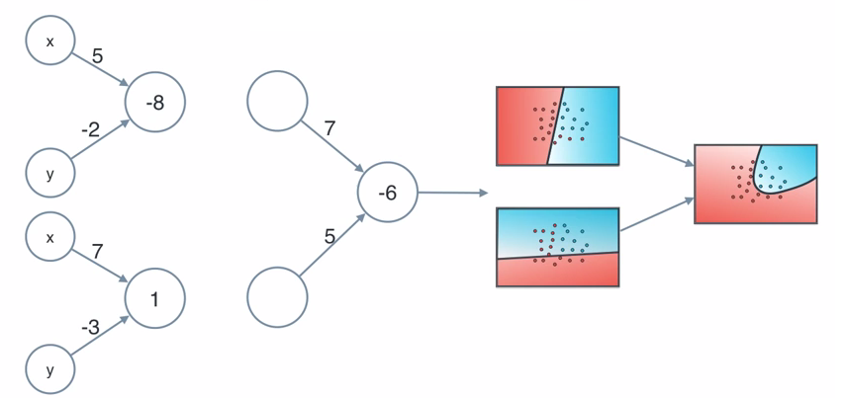
\includegraphics[width=\linewidth,keepaspectratio]{xai14}
\end{center}

\tiny{(Ref: Machine Learning - Luis Serrano - Youtube)}
\end{frame}

%%%%%%%%%%%%%%%%%%%%%%%%%%%%%%%%%%%%%%%%%%%%%%%%%%%%%%%%%%
\begin{frame}[fragile]\frametitle{How Neural Networks capture Non-Linearity?}
\begin{center}
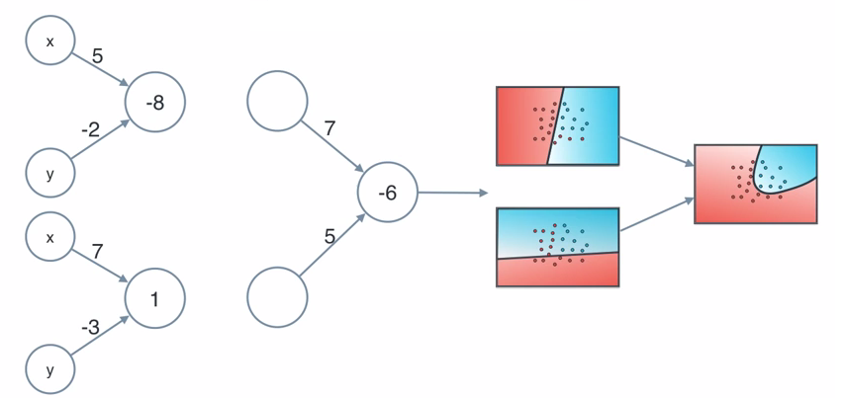
\includegraphics[width=\linewidth,keepaspectratio]{xai14}
\end{center}

\tiny{(Ref: Machine Learning - Luis Serrano - Youtube)}
\end{frame}

%%%%%%%%%%%%%%%%%%%%%%%%%%%%%%%%%%%%%%%%%%%%%%%%%%%%%%%%%%
\begin{frame}[fragile]\frametitle{How Neural Networks capture Non-Linearity?}
\begin{center}
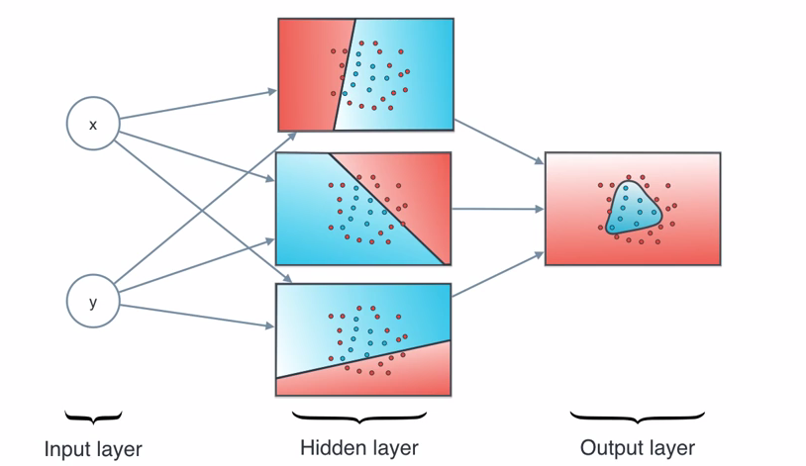
\includegraphics[width=\linewidth,keepaspectratio]{xai15}
\end{center}

\tiny{(Ref: Machine Learning - Luis Serrano - Youtube)}
\end{frame}

%%%%%%%%%%%%%%%%%%%%%%%%%%%%%%%%%%%%%%%%%%%%%%%%%%%%%%%%%%
\begin{frame}[fragile]\frametitle{The Whole Work-flow}
\begin{center}
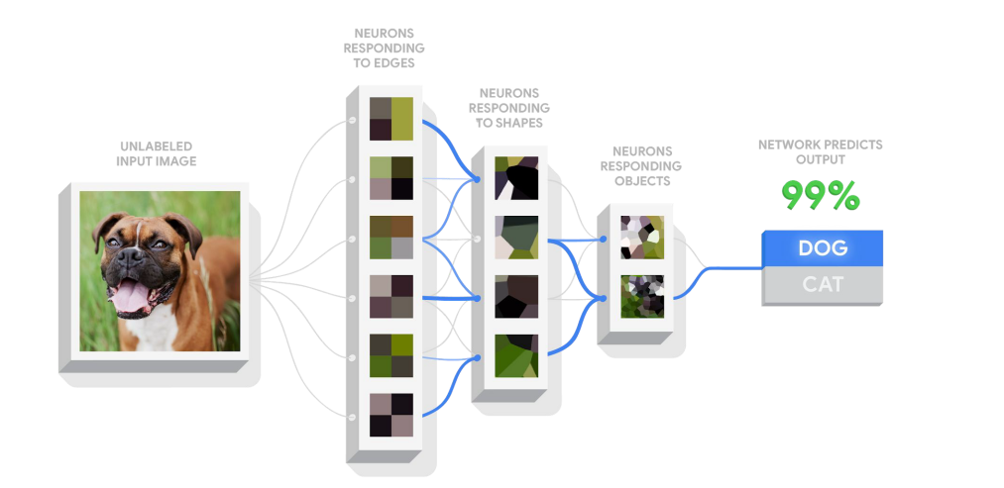
\includegraphics[width=\linewidth,keepaspectratio]{xai16}
\end{center}

\end{frame}

%%%%%%%%%%%%%%%%%%%%%%%%%%%%%%%%%%%%%%%%%%%%%%%%%%%%%%%%%%%
\begin{frame}[fragile]\frametitle{Explain-ability of AI Algorithms}
\begin{itemize}
\item {\bf Regression}: Multinomial Equation can be messy 
\item {\bf Random Forrest}: Multiple Tree and their Data Set and Voting 
\item {\bf SVM}: Kernel and Data Partition effect on Feature 
\item {\bf K Means}: Nature of Centroid don't describe cluster well. 
\item {\bf NN}: Hidden Nodes and their way of creating features 
\end{itemize}

\tiny{(Ref:Explainable AI (XAI) – A Perspective, Saurabh Kaushik  )}

\end{frame}

%%%%%%%%%%%%%%%%%%%%%%%%%%%%%%%%%%%%%%%%%%%%%%%%%%%%%%%%%%
\begin{frame}[fragile]\frametitle{But \ldots}
\begin{center}
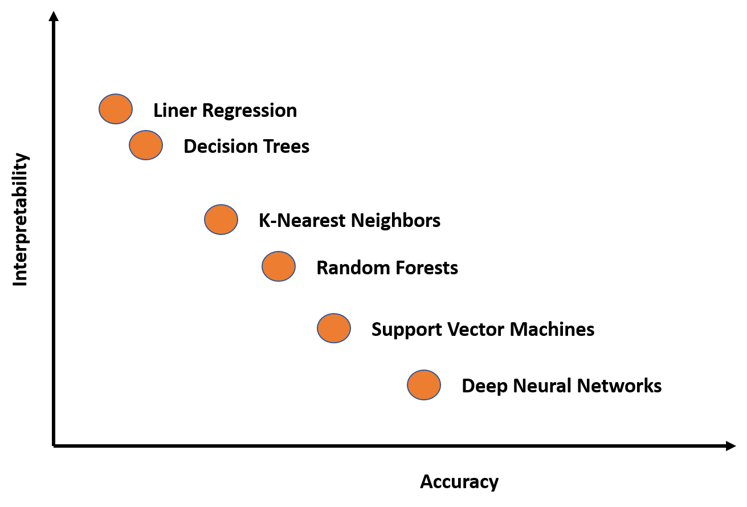
\includegraphics[width=0.8\linewidth,keepaspectratio]{xai17}
\end{center}

\tiny{(Ref: Application of artificial intelligence in gastroenterology, April 2019,World Journal of Gastroenterology 25(14):1666-1683)
}
\end{frame}


%%%%%%%%%%%%%%%%%%%%%%%%%%%%%%%%%%%%%%%%%%%%%%%%%%%%%%%%%%%%%%%%%%%%%%%%%%%%%%%%%%
\begin{frame}[fragile]\frametitle{}
\begin{center}
{\Large Techniques for Explain-ability}
\end{center}
\end{frame}

%%%%%%%%%%%%%%%%%%%%%%%%%%%%%%%%%%%%%%%%%%%%%%%%%%%%%%%%%%%
\begin{frame}[fragile]\frametitle{Types of Explain-ability}

\begin{itemize}
\item {\bf Intrinsic Methods} restrict complexity of model before training it. Selecting only some types of features, etc. {\bf Post-hoc Methods} apply after model training.
\item {\bf Model Specific Methods} are for specific types of algorithms and {\bf Model Agnostic Methods} are irrespective of algorithm type.
\item {\bf Local Methods} explain an individual prediction; {\bf Global Methods} explain the whole model behavior.
\item {\bf Visual Methods} explain via graphics.
\end{itemize}

\tiny{(Ref: XAI - Udemy  )}

\end{frame}

%%%%%%%%%%%%%%%%%%%%%%%%%%%%%%%%%%%%%%%%%%%%%%%%%%%%%%%%%%%
\begin{frame}[fragile]\frametitle{Explain-ability of AI Algorithms}
\begin{center}
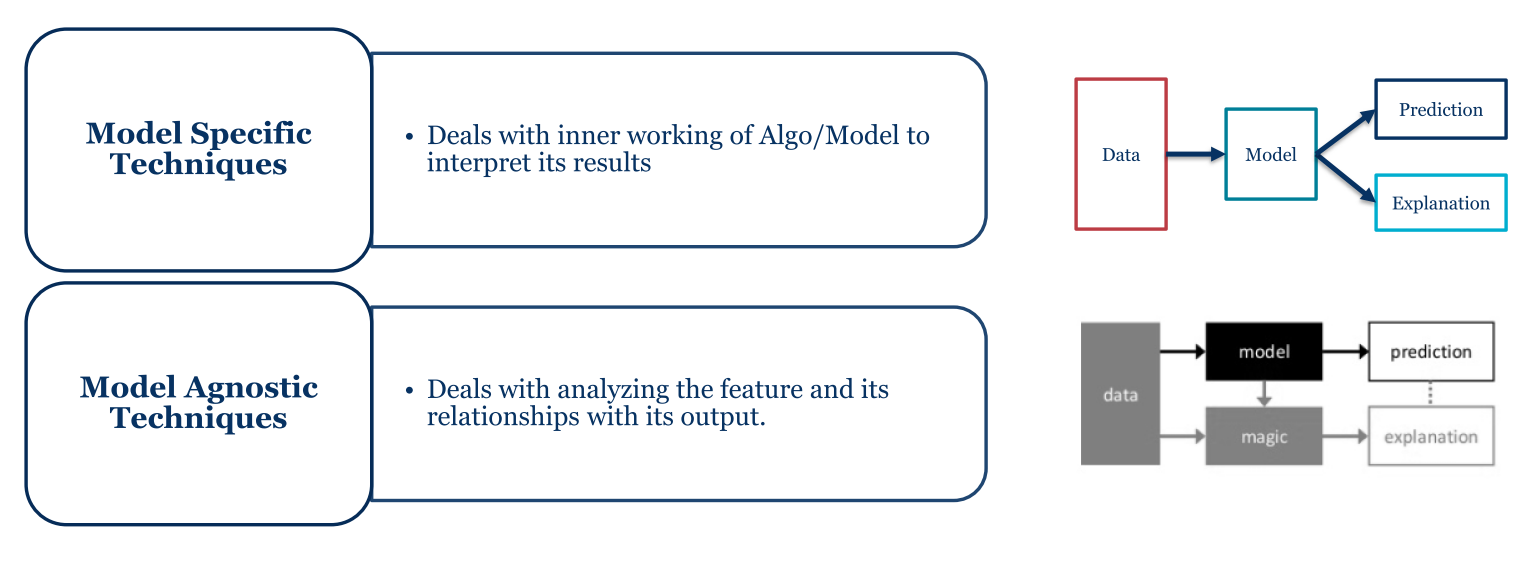
\includegraphics[width=\linewidth,keepaspectratio]{xai18}
\end{center}

\tiny{(Ref:Explainable AI (XAI) – A Perspective, Saurabh Kaushik  )}


\end{frame}

%%%%%%%%%%%%%%%%%%%%%%%%%%%%%%%%%%%%%%%%%%%%%%%%%%%%%%%%%%%
\begin{frame}[fragile]\frametitle{Model Specific vs Agnostic – Approach}
\begin{center}
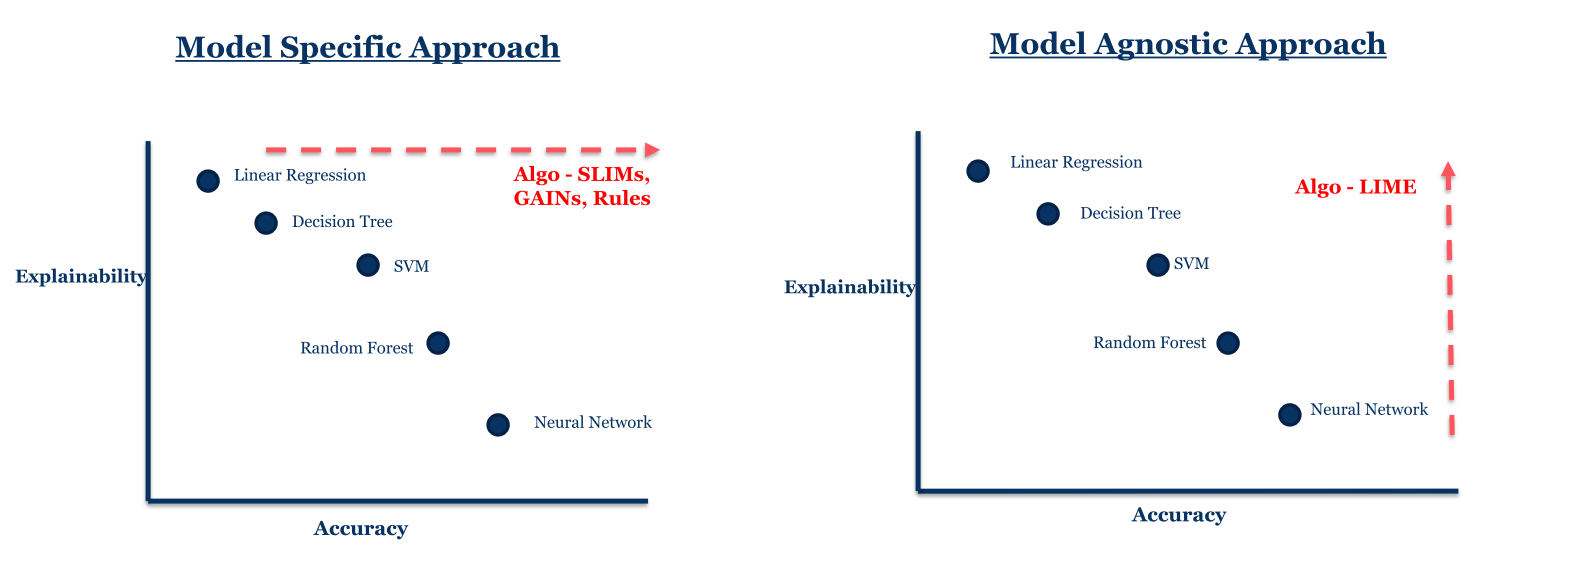
\includegraphics[width=\linewidth,keepaspectratio]{xai19}
\end{center}

\tiny{(Ref:Explainable AI (XAI) – A Perspective, Saurabh Kaushik  )}
\end{frame}

%%%%%%%%%%%%%%%%%%%%%%%%%%%%%%%%%%%%%%%%%%%%%%%%%%%%%%%%%%%
\begin{frame}[fragile]\frametitle{ Model Specific Techniques}
\begin{center}
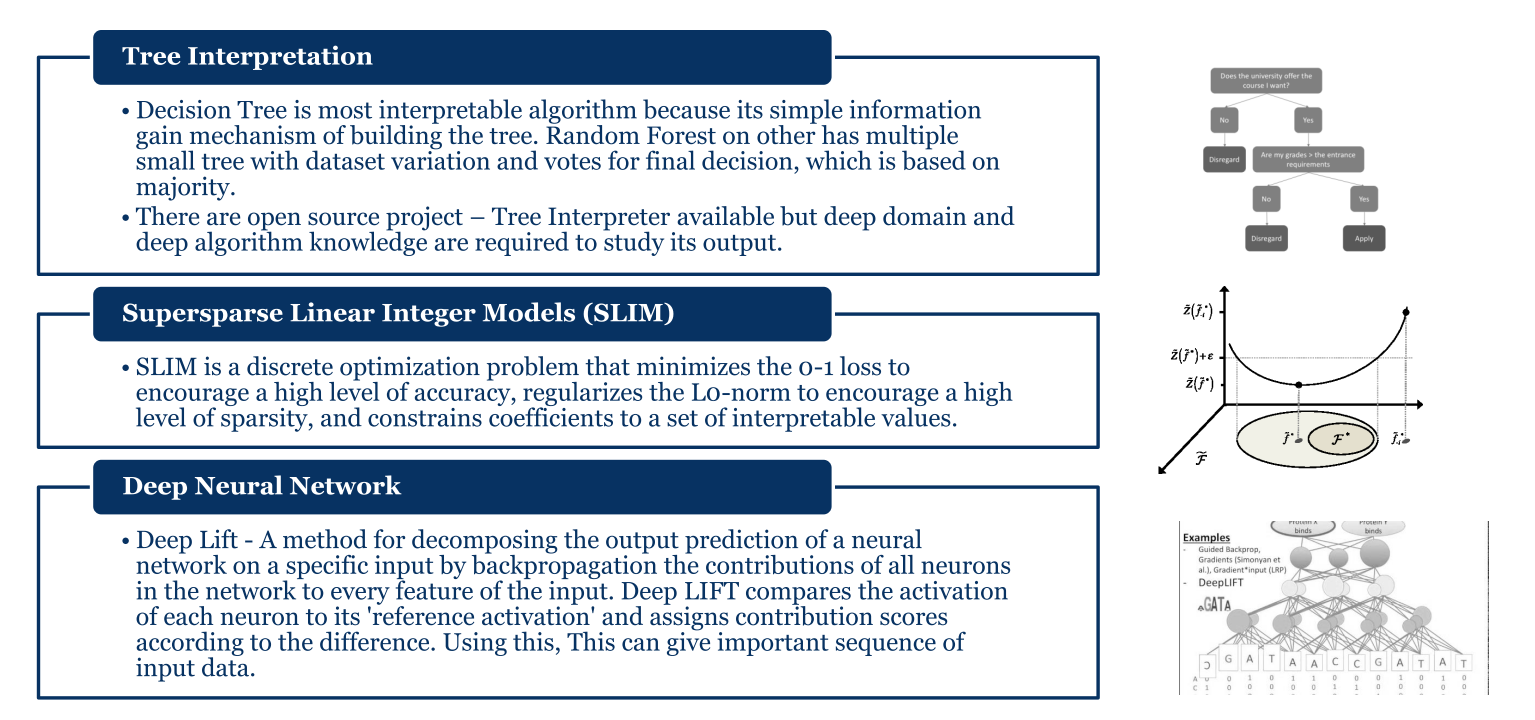
\includegraphics[width=\linewidth,keepaspectratio]{xai20}
\end{center}

\tiny{(Ref:Explainable AI (XAI) – A Perspective, Saurabh Kaushik  )}
\end{frame}

%%%%%%%%%%%%%%%%%%%%%%%%%%%%%%%%%%%%%%%%%%%%%%%%%%%%%%%%%%%
\begin{frame}[fragile]\frametitle{ Model Agnostic Techniques}
\begin{center}
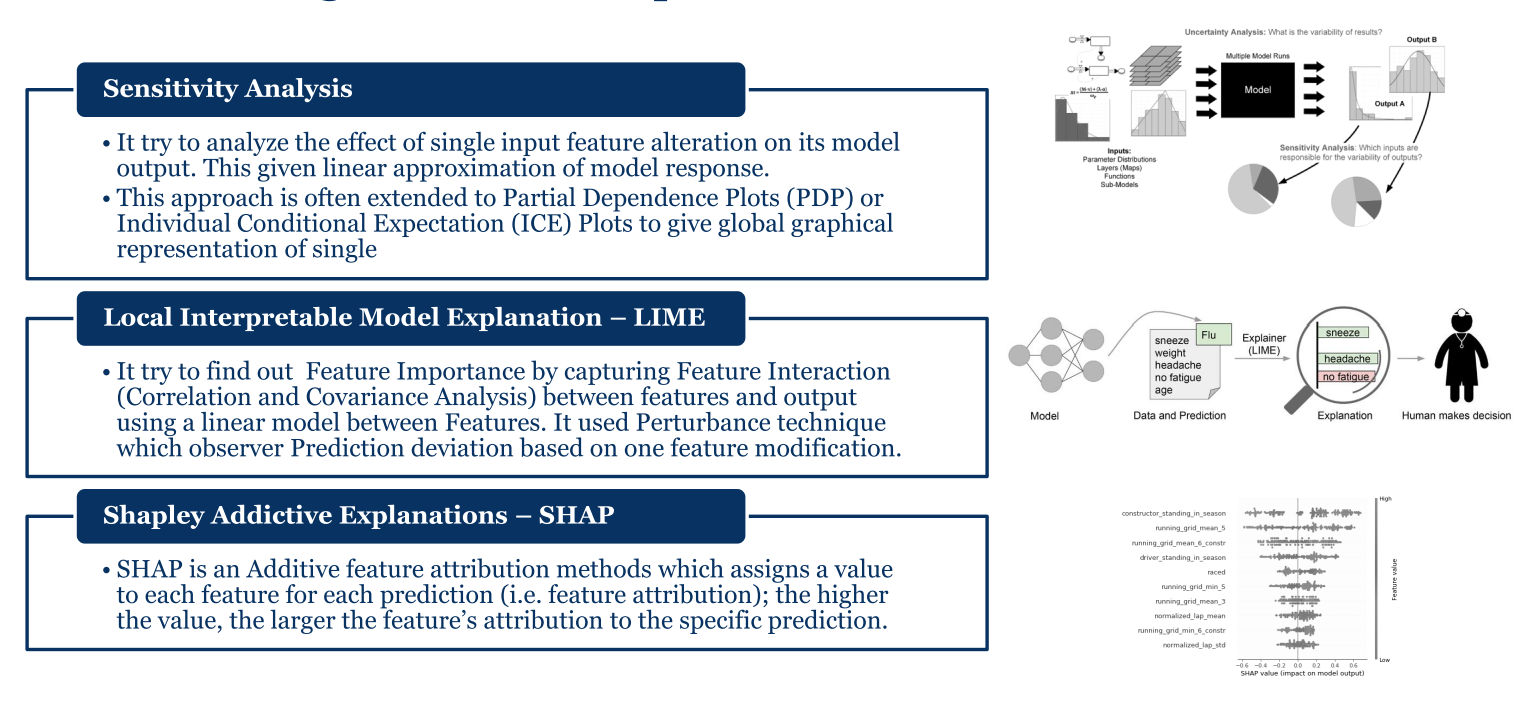
\includegraphics[width=\linewidth,keepaspectratio]{xai21}
\end{center}

\tiny{(Ref:Explainable AI (XAI) – A Perspective, Saurabh Kaushik  )}
\end{frame}

%%%%%%%%%%%%%%%%%%%%%%%%%%%%%%%%%%%%%%%%%%%%%%%%%%%%%%%%%%%
\begin{frame}[fragile]\frametitle{Summary: Types of Explain-ability}

\begin{center}
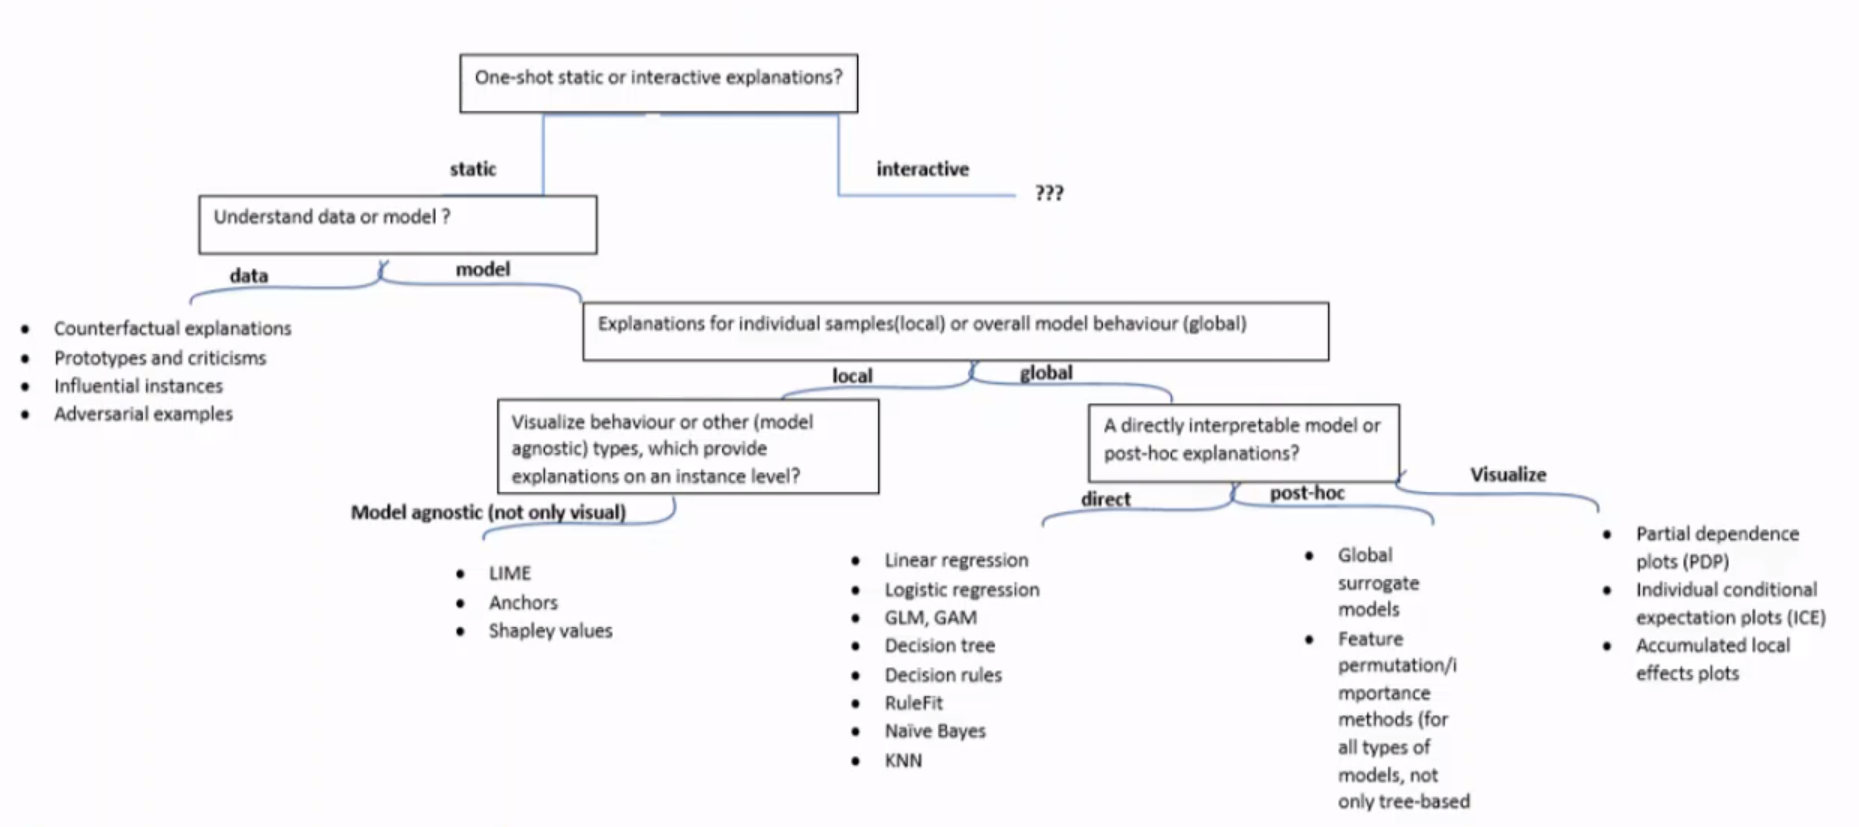
\includegraphics[width=\linewidth,keepaspectratio]{xai25}

\tiny{(Ref: XAI - Udemy  )}

\end{center}


\end{frame}


%%%%%%%%%%%%%%%%%%%%%%%%%%%%%%%%%%%%%%%%%%%%%%%%%%%%%%%%%%%%%%%%%%%%%%%%%%%%%%%%%%
\begin{frame}[fragile]\frametitle{}
\begin{center}
{\Large Conclusion}
\end{center}
\end{frame}


%%%%%%%%%%%%%%%%%%%%%%%%%%%%%%%%%%%%%%%%%%%%%%%%%%%%%%%%%%%
\begin{frame}[fragile]\frametitle{Future Techniques}
\begin{center}
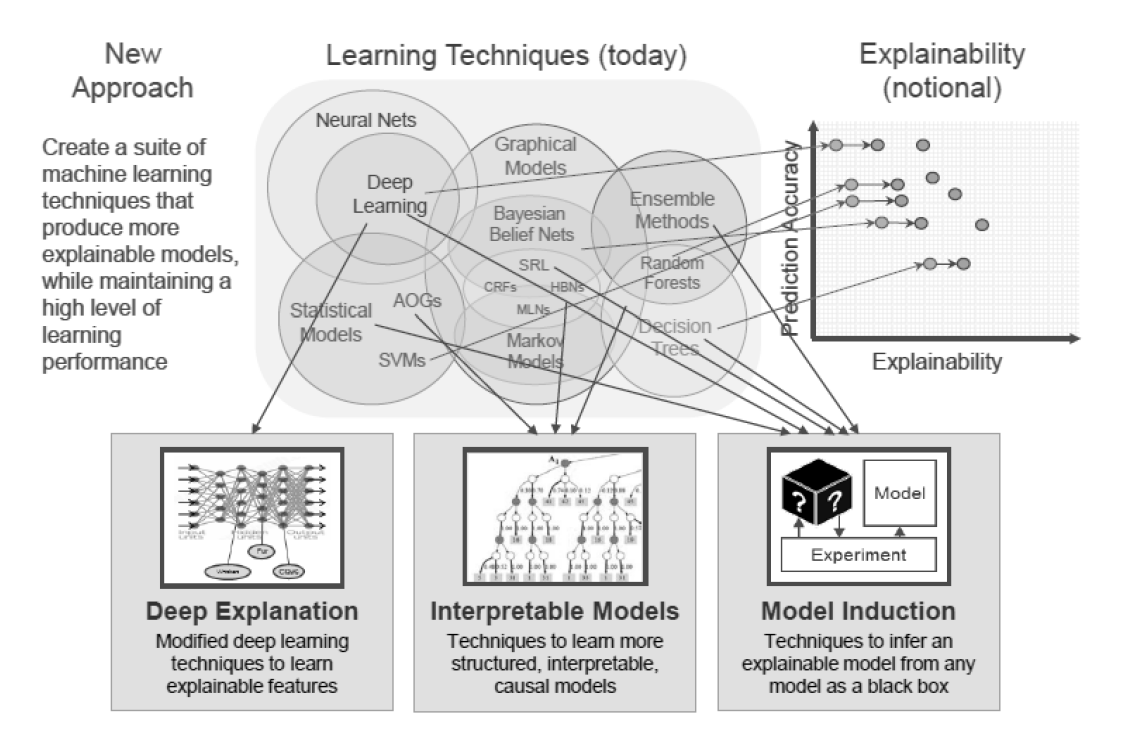
\includegraphics[width=0.8\linewidth,keepaspectratio]{xai22}
\end{center}

\tiny{(Ref:Explainable AI (XAI) – A Perspective, Saurabh Kaushik  )}
\end{frame}

%%%%%%%%%%%%%%%%%%%%%%%%%%%%%%%%%%%%%%%%%%%%%%%%%%%%%%%%%%%
\begin{frame}[fragile]\frametitle{So, Finally \ldots}

\begin{center}
AI is just a set of algorithms, 
which (predominantly ) finds patterns from given Inputs as well as Outputs
\end{center}
\end{frame}

%%%%%%%%%%%%%%%%%%%%%%%%%%%%%%%%%%%%%%%%%%%%%%%%%%%%%%%%%%%
\begin{frame}[fragile]\frametitle{For example: to find out clause ``Term'' \ldots}
\begin{itemize}
\item Need to supply AI algorithm with 100s/1000s of ``Term'' clause samples
\item Gets trained on patterns, word frequencies, context words
\item Stores this information as ``model''
\item Can be used to classify unseen clause, whether ``Term'' or not.
\end{itemize}
\end{frame}

%%%%%%%%%%%%%%%%%%%%%%%%%%%%%%%%%%%%%%%%%%%%%%%%%%%%%%%%%%%
\begin{frame}[fragile]\frametitle{Quiz}
If you want to find something ``new'', what would be needed?
\end{frame}

%%%%%%%%%%%%%%%%%%%%%%%%%%%%%%%%%%%%%%%%%%%%%%%%%%%%%%%%%%%
\begin{frame}[fragile]\frametitle{Summary}
\begin{itemize}
\item AI-ML-DL approaches are non-deterministic (but (\ldots)?)
\item For good results, need good annotated data and lots of it
\item Annotations need to be perfect (``Gold''), else Garbage-In-(\ldots)
\item Data should cover all possible variations
\item AI-ML-DL just fits the data, but just that, it does it automatically!!
\item ML has better explain-ability than DL (why?)
\end{itemize}
\end{frame}

%%%%%%%%%%%%%%%%%%%%%%%%%%%%%%%%%%%%%%%%%%%%%%%%%%%%%%%%%%%
\begin{frame}[fragile]\frametitle{Btw, thoughts to ponder on \ldots}
\begin{itemize}
\item ‘AI is biased'
\item ‘Explainable AI' is to understand how/why it is biased
\item But then \ldots
\item Human are biased too \ldots
\item ‘Explainable Humans'\ldots the next topic?
\end{itemize}
\end{frame}
